\section{Experiment 1: Horizontal and vertical bars}
\label{section:horvertAdaptiveInhibition}

\subsection{Introduction}

For this experiment images of either horizontal or vertical bars were shown to the WTA network. The network trained its weights through unsupervised learning. Through that, it learned to cluster the images together, depending on the orientation and position of the bars. The learning of the network was visualized and analysed.
Further, the effect of the prior neurons was demonstrated. Ambiguous images, which showed a horizontal and a vertical bar at the same time, were generated and given to the network. Through that, the network's capability to shift its attention to specific parts of the image, depending on the prior was demonstrated.

\subsection{Methods}

\paragraph{Input data}
Black bars, with a width of seven pixels, were drawn onto a white background, with a size of 35 x 35 pixels. The bars could be oriented either horizontally or vertically and be shifted in position. The network was supposed to identify ten different groups within these images, five with a horizontal orientation and five with a vertical orientation. With a chosen bar width of seven pixels the image height and width were determined as 35 pixels, as five bars should have place next to each other, without overlap, in each orientation. Each of those bars represented one group of bars. Thus, each group had a size of seven pixels. Starting to count from position 0, the centers of the groups should be at positions 3, 10, 17, 24, 31. The orientation of the training images was chosen randomly, via a uniform distribution. The positions of the bars in the training images were also distributed randomly, via a uniform distribution, along the 35 pixels of either axis. To simulate noise, each pixel of an image had a chance of ten percent to have its color flipped after the generation.
During the training of the network, random images were generated and presented for 200 ms. As the simulation had a duration of 800 seconds this resulted in 4000 images, which were shown to the network. Examples of the input data can be seen in Figure \ref{fig:horvertImages}. To show the value of the added a-priori information, validation images with two bars forming a cross were also generated, seen in Figure \ref{fig:horvertTrainingCrossImage}. When shown to the network in the validation process the prior neurons were given the information that a cross is either of horizontal or vertical orientation.

\begin{figure}
  \includegraphics[width=\linewidth]{figures/horvert/horvertTrainingImages.png}
  \caption{Generated training images. One image of each possible orientation at a random position.}
  \label{fig:horvertImages}
\end{figure}

\begin{figure}
\centering
  \includegraphics[width=0.45\linewidth]{figures/horvert/horvertTrainingCrossImage.png}
  \caption{Generated cross image, which can represent either horizontal or vertical orientation.}
  \label{fig:horvertTrainingCrossImage}
\end{figure}

\paragraph{Network architecture}

The network had 2450 input neurons, as every pixel of an image was connected to two input neurons. The first neuron of each pixel was in an active state, if the pixel was black and the second neuron was active, if the pixel was white. Each of these neurons had a firing frequency $f_{input}$ of 20 Hz, when in the active state and 0 Hz otherwise. Then there were ten output neurons, one for each possible group. Lastly, there were two equal sized groups of prior neurons with firing frequencies $f_{prior}$ of 200 Hz. This firing frequency was assigned a high plausible value to keep the needed number of prior neurons small compared to the number of input neurons. During training, the first group $z^h$ was active when the image was of horizontal orientation and the other group $z^v$ was active for vertical orientation. Just like the input images' pixels, the prior had a chance of 10 percent to flip. The number of prior neurons had to be determined via grid search, as they needed to be set at values, where the impact of the a-priori information is neither too strong, nor too weak.

\paragraph{Network and hyperparameters}

The simulation of the experiment was performed in time steps of 1 ms. This step size was used for all experiments. As given by \citet{nessler} the time window $\sigma$ was 10 ms, the time constant for the rise of the EPSPs $\tau_{rise}$ was 1 ms and the time constant for the decay of the EPSPs $\tau_{decay}$ was 15 ms. Before performing this experiment, Experiment 2 of \citet{nessler} was reproduced to validate that the implementation of the simulation was correct. This proof of concept was omitted in this work, however, within it the weight shift hyperparameter $c = 20$ and the learning rate $\lambda = 10^{-3}$ were determined via grid search. These hyperparameter values were reused for this experiment as the input data, as well as the network architecture, were similar.

\subsection{Results}

First, different numbers of prior neurons were tested. Simulations with 10, 20, 50, 100 and 200 prior neurons were performed. For 50, 100 and 200 prior neurons the training process was impaired, by the activity of the prior neurons. Some output neurons were responding to too large areas, while other prior neurons were not responding to any specific areas at all. This happened, for example, because the first output neuron that generated a spike for a horizontal bar got reinforced by the prior neurons to respond to all horizontal bars, no matter the position. Thus, other output neurons were less likely to respond to horizontal bars, resulting in output neurons that were not responding to any specific orientation or area at all. With a number of 10 and 20 prior neurons, each of the output neurons learned to respond to coherent areas of the images. The prior neurons also learned to respond to either horizontal or vertical images. To maximize the impact of the a-priori information the validation of the network was performed with 20 prior neurons, as it was the largest number that resulted in a properly trained network. The results of the training process can be seen in Figure \ref{fig:horvertAdaptiveInhibitionTraining}. In Figure \ref{fig:horvertAdaptiveInhibitionTraining}A examples of input images are shown. The bars were positioned without overlapping each other, thus showing the optimal areas output neurons should learn to respond to. The areas that output neurons did learn to respond to, can be seen in the visualization of the input weights in Figure \ref{fig:horvertAdaptiveInhibitionTraining}B. It can be seen, that the training was successful, as five output neurons responded to horizontal bars and the other five to vertical bars. Furthermore, each output neuron responded to different areas of the input image and there was little overlap between each other. The training progress of the network is given in Figure \ref{fig:horvertAdaptiveInhibitionTraining}E. When the network has completed the training it should mostly have only one or two output neurons being active for any input image. Although, there may be more active output neurons sporadically, due to the stochastic nature of the model. According to this plot, the training process could have been stopped earlier after 2000 shown images. However, as there was no danger of overfitting the data, more images were shown, to ensure that the network had always finished the training when the simulation stopped. In Figure \ref{fig:horvertAdaptiveInhibitionTraining}F the relative activity of the most active output neuron can be seen. First, it can also be used to judge the progress of the training process, as it increased over time. Furthermore, it can also be seen as a measure of how clearly an image belonged to the area the most active output neuron responded to. If the position of an image was exactly in the middle of the learned area of the most active output neuron, then the relative activity should be one. However, when the position was on the border between two learned areas of output neurons, then the relative activity should only be 0.5, as the image belonged to both areas. The learned prior weights can be seen in Figure \ref{fig:horvertAdaptiveInhibitionpriorWeights}. There it can be seen, that the first 10 prior neurons learned the same pattern, as all of them were in an active state whenever vertical bars were shown to the network. When comparing these prior weights to the input weights in Figure \ref{fig:horvertAdaptiveInhibitionTraining}B it can be seen that the five highest prior weights of each prior neuron are between themselves and output neurons that learned to respond to vertical bars. The last 10 prior weights showed exactly the opposite pattern, having their five highest weight values between themselves and output neurons that responded to horizontal bars.

\begin{figure}
  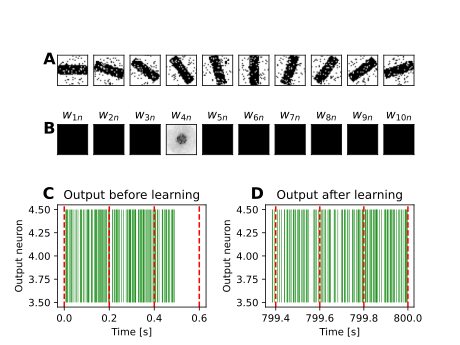
\includegraphics[width=\linewidth]{figures/horvertAdaptiveInh/trainingPlot.png}
  \caption{\textbf{Training with 20 prior neurons.} \textbf{A} Examples of 35 x 35-pixel input images of horizontal and vertical bars with background noise. They were positioned without overlapping each others bars, thus showing the optimal areas output neurons should learn to respond to. \textbf{B} Learned weights of the connections between the input neurons, that were active for black pixels of the input image, and output neurons. As there was one such input neuron per pixel of the image the weights could be plotted in the same format as the image to easily interpret them. \textbf{C, D} Spike activity expressed by the output neurons before and after the training of the network. \textbf{E} Number of active output neurons during the presentation duration of each training image. \textbf{F} This shows the number of spikes the most active output neuron generated, relative to the number of spikes all other output neurons generated combined. }
  \label{fig:horvertAdaptiveInhibitionTraining}
\end{figure}

\begin{figure}
  \includegraphics[width=\linewidth]{figures/horvertAdaptiveInh/priorWeights.png}
  \caption{ Learned weights of the connections between prior and output neurons. }
  \label{fig:horvertAdaptiveInhibitionpriorWeights}
\end{figure}

To validate the learned patterns, the network was shown horizontal bars with a height of seven pixels, with their centers at every possible position, beginning at position zero and incrementing in steps of one. Each image was shown for 200 ms each, while recording the output neuron activity. To visualize which output neuron is the most active for each position, a horizontal bar with a height of one was drawn into a 35 x 35 pixel image, color-coded to represent the most active output neuron for that position. This can be seen in Figure \ref{fig:horvertAdaptiveInhibitionHorizontalValResults}A. $y_7$ and $y_{10}$ claimed areas with heights of eight pixels, while the areas of $y_9$ and $y_4$ had only a height of six pixels. Only $y_2$ had an area height of the expected seven pixels. These varying heights were expected to happen, due to the stochastic nature of the model and the unsupervised learning method applied in this thesis. Depending on the randomly generated images the network received during the training process, there may be more images on one side of the border between two output neurons, than on the other side. This would result in the favoured neuron having stronger weights around the border area. Because of that, the favoured neuron might end up claiming a larger active area.
The output spikes of the network can be seen in Figure  \ref{fig:horvertAdaptiveInhibitionHorizontalValResults}B. It can be seen, that outside of the border areas between the output neurons there was mostly only one neuron active. However, shortly after two seconds $y_8$ was active. The time frame between 2 seconds and 2.2 seconds corresponds to position 10. $y_8$ should mostly be active for vertical bars, however, its learned area has some overlap with a horizontal bar at position ten and thus there is always a small chance for it to generate a spike. 
In Figure \ref{fig:horvertAdaptiveInhibitionHorizontalValResults}C the number of active output neurons for each position is given.  The validation process was repeated ten times and the mean and standard deviation of the number were calculated. In this plot four peaks appeared. These peaks are around the borders between the adjacent active areas of output neurons seen in Figure \ref{fig:horvertAdaptiveInhibitionHorizontalValResults}A. Around the border areas a number of active output neurons bigger than one was expected, as the horizontal bars reach into the areas of two output neurons at once. When looking at the number of active output neurons at position 10, which is approximately 1.1 with a high standard deviation, it shows that $y_8$ did not falsely learn to be active for horizontal bars, but rather that it was a stochastic outlier. Figure \ref{fig:horvertAdaptiveInhibitionHorizontalValResults}D shows the relative activity of the most active output neuron. Compared to Figure \ref{fig:horvertAdaptiveInhibitionHorizontalValResults}C, it provides the additional information of how split the activity of neighbouring output neurons is in the border areas. For example, it can be seen that at position 22 $y_4$ had a relative activity of 0.62. It was only barely able to be the most active neuron and might almost have had only an active area with a height of five pixels.

\begin{figure}
  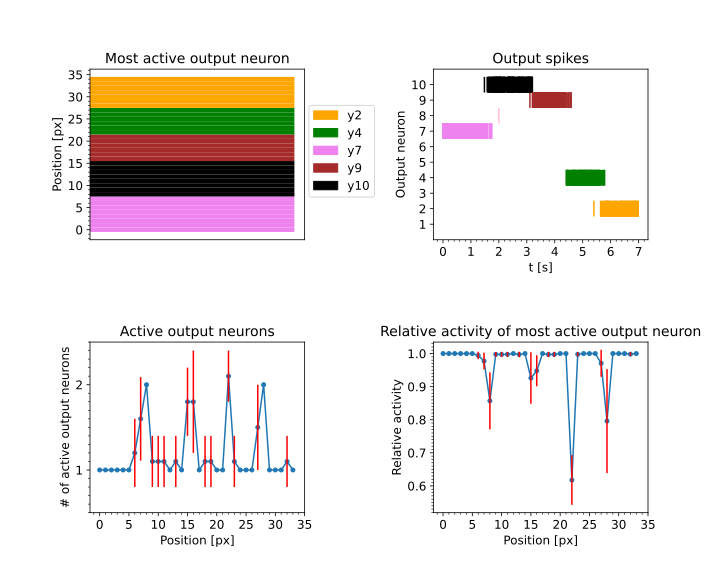
\includegraphics[width=\linewidth]{figures/horvertAdaptiveInh/horizontal_validation.png}
  \caption{\textbf{Horizontal validation.} Horizontal bars with a height of seven pixels were shown to the network at different positions. \textbf{A} Most active output neuron, depending on the vertical position of the center of a horizontal bar. \textbf{B} Output spikes during the validation process. The ticks of the x-axis are in steps of 0.2 seconds, thus each tick signifies the start of a new image being shown. \textbf{C} The mean number of active output neurons, depending on the vertical position of a horizontal bar. The standard deviation is given by the red bars. \textbf{D} This shows the number of spikes that the most active output neuron generated, relative to the number of spikes all other output neurons generated combined. The blue dots indicate the mean and the red bars the standard deviation. }
  \label{fig:horvertAdaptiveInhibitionHorizontalValResults}
\end{figure}

The validation process for the vertical bars was done analogously to the horizontal bars. Its results are given in Figure \ref{fig:horvertAdaptiveInhibitionVerticalValResults}. 
 
\begin{figure}
  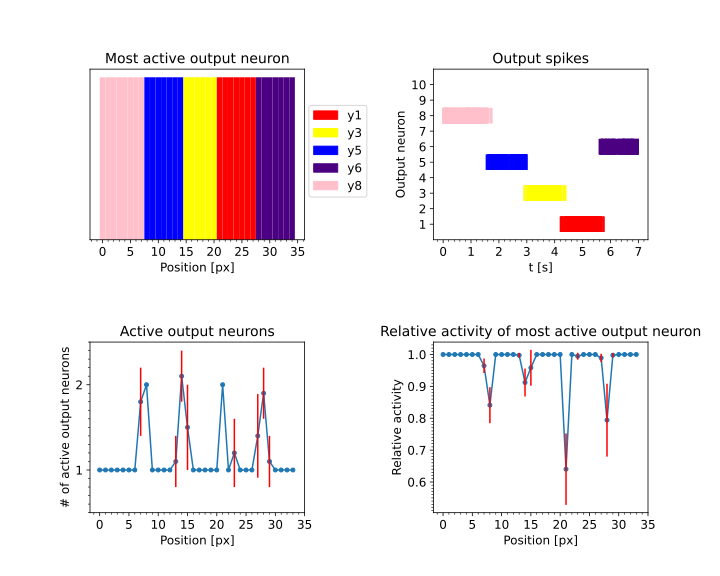
\includegraphics[width=\linewidth]{figures/horvertAdaptiveInh/vertical_validation.png}
  \caption{\textbf{Vertical validation.} Vertical bars with a height of seven pixels were shown to the network at different positions. \textbf{A} Most active output neuron, depending on the horizontal position of the center of a vertical bar. \textbf{B} Output spikes during the validation process. The ticks of the x-axis are in steps of 0.2 seconds, thus each tick signifies the start of a new image being shown. \textbf{C} The mean number of active output neurons, depending on the horizontal position of a vertical bar. The standard deviation is given by the red bars. \textbf{D} This shows the number of spikes that the most active output neuron generated, relative to the number of spikes all other output neurons generated combined. The blue dots indicate the mean and the red bars the standard deviation. }
  \label{fig:horvertAdaptiveInhibitionVerticalValResults}
\end{figure}

Next, the impact of the prior was analysed. An image with a horizontal bar at position 12 and a vertical bar at position 5 on it was generated. First, the prior neurons $z^v$ were activated and $z^h$ were deactivated. Then the image was shown to the network for 200 ms. After that the activity of the prior neurons was reversed and the image was shown again. The results can be seen in Figure \ref{fig:horvertAdaptiveInhibitionPriorValResults}. In that figure it can be seen, that the output of the network completely changes, depending of the prior activity. The prior neurons determine if the network focuses on the vertical or horizontal bar of the image.

\begin{figure}
  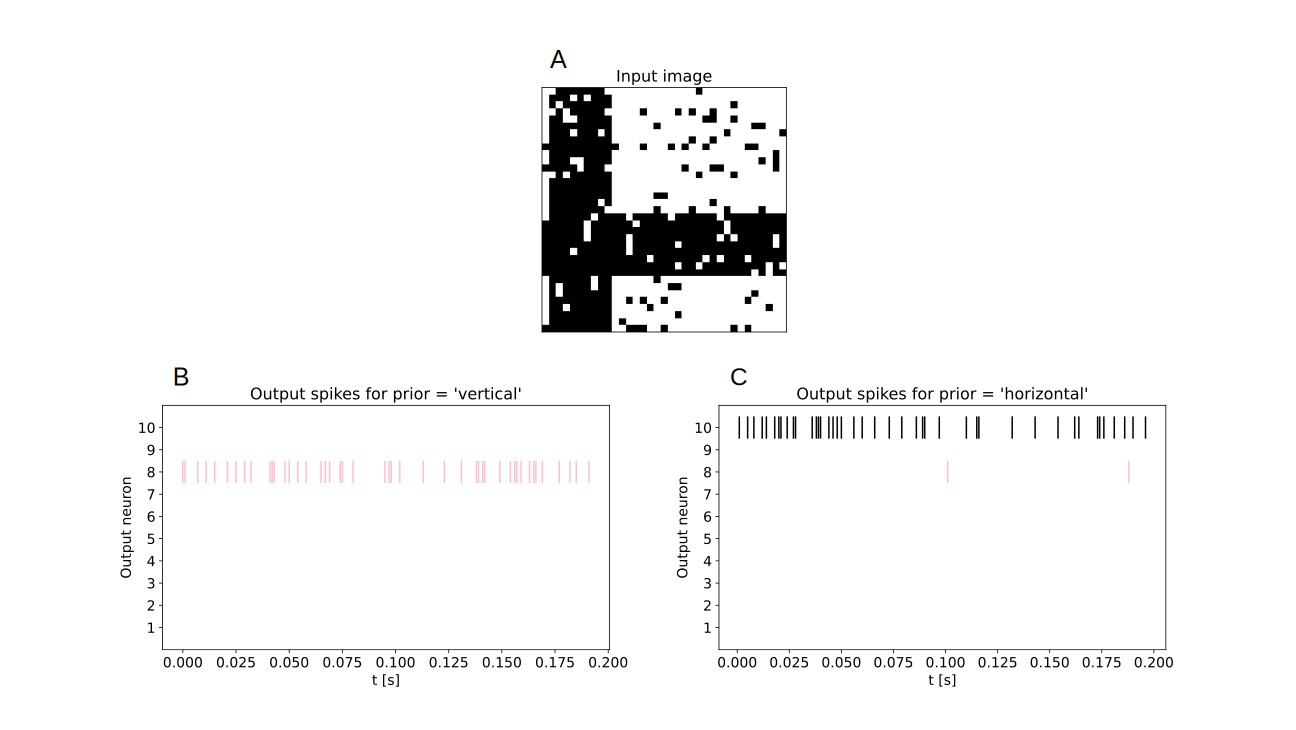
\includegraphics[width=\linewidth]{figures/horvertAdaptiveInh/20priors_pos5and12/crossValidation.png}
  \caption{\textbf{Impact of the prior Neurons.} \textbf{A} Validation image with a horizontal and a vertical bar on it. \textbf{B} Spiking activity of the output neurons with $z^v$ being active. \textbf{C} Spiking activity of the output neurons with $z^h$ being active. }
  \label{fig:horvertAdaptiveInhibitionPriorValResults}
\end{figure}

To further illustrate the dependence of the output on the prior, the firing frequencies of the prior neurons were gradually changed. The starting firing frequency of $z^h$ was set to 200 Hz and to 0 Hz for $z^v$. For those firing frequencies a cross image was shown to the network for 200 ms. It had a horizontal bar at position 31 and a vertical bar at position 3. These position are as far at the edge of the image as possible, while still displaying the whole width of the bars. After each image presentation duration the firing frequency of $z^h$ was decreased by 1 Hz and increased by 1 Hz for $z^v$. The used cross image can be seen in Figure \ref{fig:horvertAdaptiveInhibitionVariablePriorResults}A. The firing frequency of the 2 most active output neurons, depending on the firing frequency of $z^v$, can be seen in Figure \ref{fig:horvertAdaptiveInhibitionVariablePriorResults}B. At the beginning $y_2$, which represents the horizontal part of the cross image, was the most active neuron, which is correct as the prior neurons fully supported the horizontal interpretation of the input image. With rising firing frequency of $z^v$, the activity of $y_2$ decreased and the activity of $y_8$ increased. This happened, because the prior neurons gradually supported the interpretation of the image as vertical more and more. It was expected, that the crossing point of the two graphs in Figure \ref{fig:horvertAdaptiveInhibitionVariablePriorResults}B would be at a firing frequency of $z^v$ of 100 Hz, however, the graphs crossed at 58.6 Hz. In Figure \ref{fig:horvertAdaptiveInhibitionHorizontalValResults}D the relative activity of $y_2$ at the edge of the bar, at position 28, was 0.79. In Figure \ref{fig:horvertAdaptiveInhibitionVerticalValResults}D the relative activity of $y_8$ at the edge of the bar, at position 6, was 1.0. $y_8$ has a higher relative activity at that position than $y_2$ at position 28, because $y_8$ has an  active area of width 8, making position 6 not the border of the active area. Due to the larger active area of $y_8$ the crossing point shifted in favour of $y_8$.

\begin{figure}
  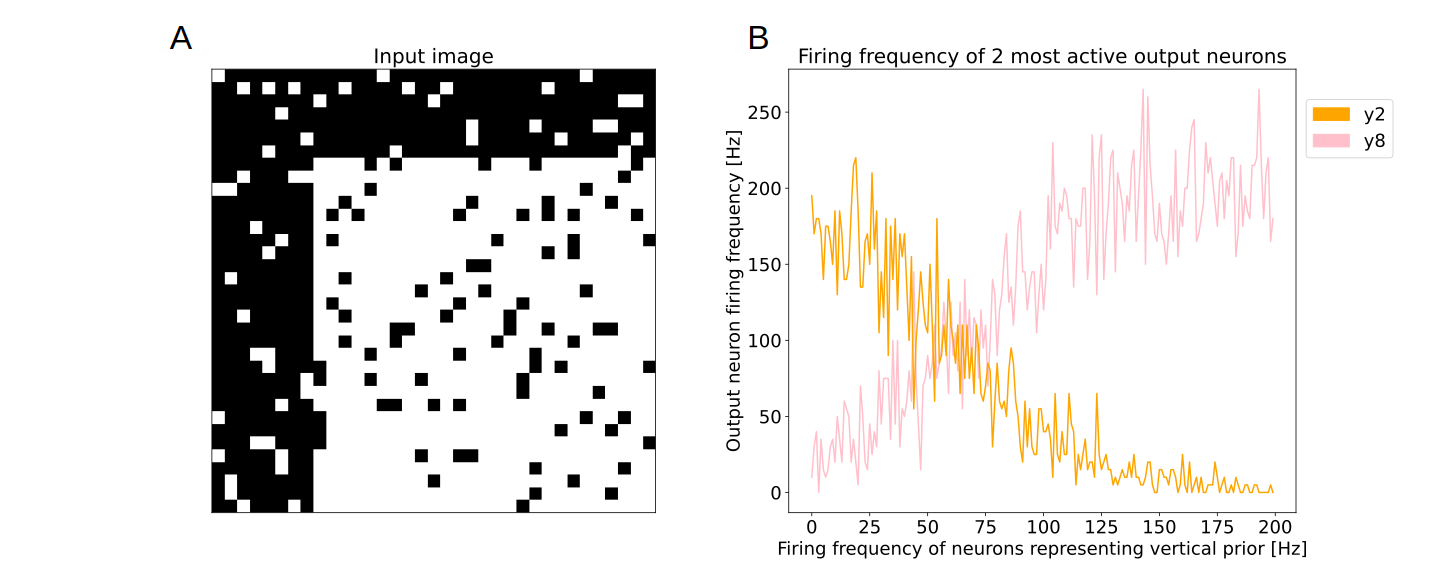
\includegraphics[width=\linewidth]{figures/horvertAdaptiveInh/YFrequency_prior.png}
  \caption{\textbf{Cross image with varying prior neuron activity.} \textbf{A} Validation cross image. \textbf{B} Firing frequency of the 2 most active output neurons, depending on the firing frequency of $z^v$. The output neuron firing frequencies were averaged over 10 runs to smooth the graphs.}
  \label{fig:horvertAdaptiveInhibitionVariablePriorResults}
\end{figure}
